\documentclass[1p]{elsarticle_modified}
%\bibliographystyle{elsarticle-num}

%\usepackage[colorlinks]{hyperref}
%\usepackage{abbrmath_seonhwa} %\Abb, \Ascr, \Acal ,\Abf, \Afrak
\usepackage{amsfonts}
\usepackage{amssymb}
\usepackage{amsmath}
\usepackage{amsthm}
\usepackage{scalefnt}
\usepackage{amsbsy}
\usepackage{kotex}
\usepackage{caption}
\usepackage{subfig}
\usepackage{color}
\usepackage{graphicx}
\usepackage{xcolor} %% white, black, red, green, blue, cyan, magenta, yellow
\usepackage{float}
\usepackage{setspace}
\usepackage{hyperref}

\usepackage{tikz}
\usetikzlibrary{arrows}

\usepackage{multirow}
\usepackage{array} % fixed length table
\usepackage{hhline}

%%%%%%%%%%%%%%%%%%%%%
\makeatletter
\renewcommand*\env@matrix[1][\arraystretch]{%
	\edef\arraystretch{#1}%
	\hskip -\arraycolsep
	\let\@ifnextchar\new@ifnextchar
	\array{*\c@MaxMatrixCols c}}
\makeatother %https://tex.stackexchange.com/questions/14071/how-can-i-increase-the-line-spacing-in-a-matrix
%%%%%%%%%%%%%%%

\usepackage[normalem]{ulem}

\newcommand{\msout}[1]{\ifmmode\text{\sout{\ensuremath{#1}}}\else\sout{#1}\fi}
%SOURCE: \msout is \stkout macro in https://tex.stackexchange.com/questions/20609/strikeout-in-math-mode

\newcommand{\cancel}[1]{
	\ifmmode
	{\color{red}\msout{#1}}
	\else
	{\color{red}\sout{#1}}
	\fi
}

\newcommand{\add}[1]{
	{\color{blue}\uwave{#1}}
}

\newcommand{\replace}[2]{
	\ifmmode
	{\color{red}\msout{#1}}{\color{blue}\uwave{#2}}
	\else
	{\color{red}\sout{#1}}{\color{blue}\uwave{#2}}
	\fi
}

\newcommand{\Sol}{\mathcal{S}} %segment
\newcommand{\D}{D} %diagram
\newcommand{\A}{\mathcal{A}} %arc


%%%%%%%%%%%%%%%%%%%%%%%%%%%%%5 test

\def\sl{\operatorname{\textup{SL}}(2,\Cbb)}
\def\psl{\operatorname{\textup{PSL}}(2,\Cbb)}
\def\quan{\mkern 1mu \triangleright \mkern 1mu}

\theoremstyle{definition}
\newtheorem{thm}{Theorem}[section]
\newtheorem{prop}[thm]{Proposition}
\newtheorem{lem}[thm]{Lemma}
\newtheorem{ques}[thm]{Question}
\newtheorem{cor}[thm]{Corollary}
\newtheorem{defn}[thm]{Definition}
\newtheorem{exam}[thm]{Example}
\newtheorem{rmk}[thm]{Remark}
\newtheorem{alg}[thm]{Algorithm}

\newcommand{\I}{\sqrt{-1}}
\begin{document}

%\begin{frontmatter}
%
%\title{Boundary parabolic representations of knots up to 8 crossings}
%
%%% Group authors per affiliation:
%\author{Yunhi Cho} 
%\address{Department of Mathematics, University of Seoul, Seoul, Korea}
%\ead{yhcho@uos.ac.kr}
%
%
%\author{Seonhwa Kim} %\fnref{s_kim}}
%\address{Center for Geometry and Physics, Institute for Basic Science, Pohang, 37673, Korea}
%\ead{ryeona17@ibs.re.kr}
%
%\author{Hyuk Kim}
%\address{Department of Mathematical Sciences, Seoul National University, Seoul 08826, Korea}
%\ead{hyukkim@snu.ac.kr}
%
%\author{Seokbeom Yoon}
%\address{Department of Mathematical Sciences, Seoul National University, Seoul, 08826,  Korea}
%\ead{sbyoon15@snu.ac.kr}
%
%\begin{abstract}
%We find all boundary parabolic representation of knots up to 8 crossings.
%
%\end{abstract}
%\begin{keyword}
%    \MSC[2010] 57M25 
%\end{keyword}
%
%\end{frontmatter}

%\linenumbers
%\tableofcontents
%
\newcommand\colored[1]{\textcolor{white}{\rule[-0.35ex]{0.8em}{1.4ex}}\kern-0.8em\color{red} #1}%
%\newcommand\colored[1]{\textcolor{white}{ #1}\kern-2.17ex	\textcolor{white}{ #1}\kern-1.81ex	\textcolor{white}{ #1}\kern-2.15ex\color{red}#1	}

{\Large $\underline{12n_{0021}~(K12n_{0021})}$}

\setlength{\tabcolsep}{10pt}
\renewcommand{\arraystretch}{1.6}
\vspace{1cm}\begin{tabular}{m{100pt}>{\centering\arraybackslash}m{274pt}}
\multirow{5}{120pt}{
	\centering
	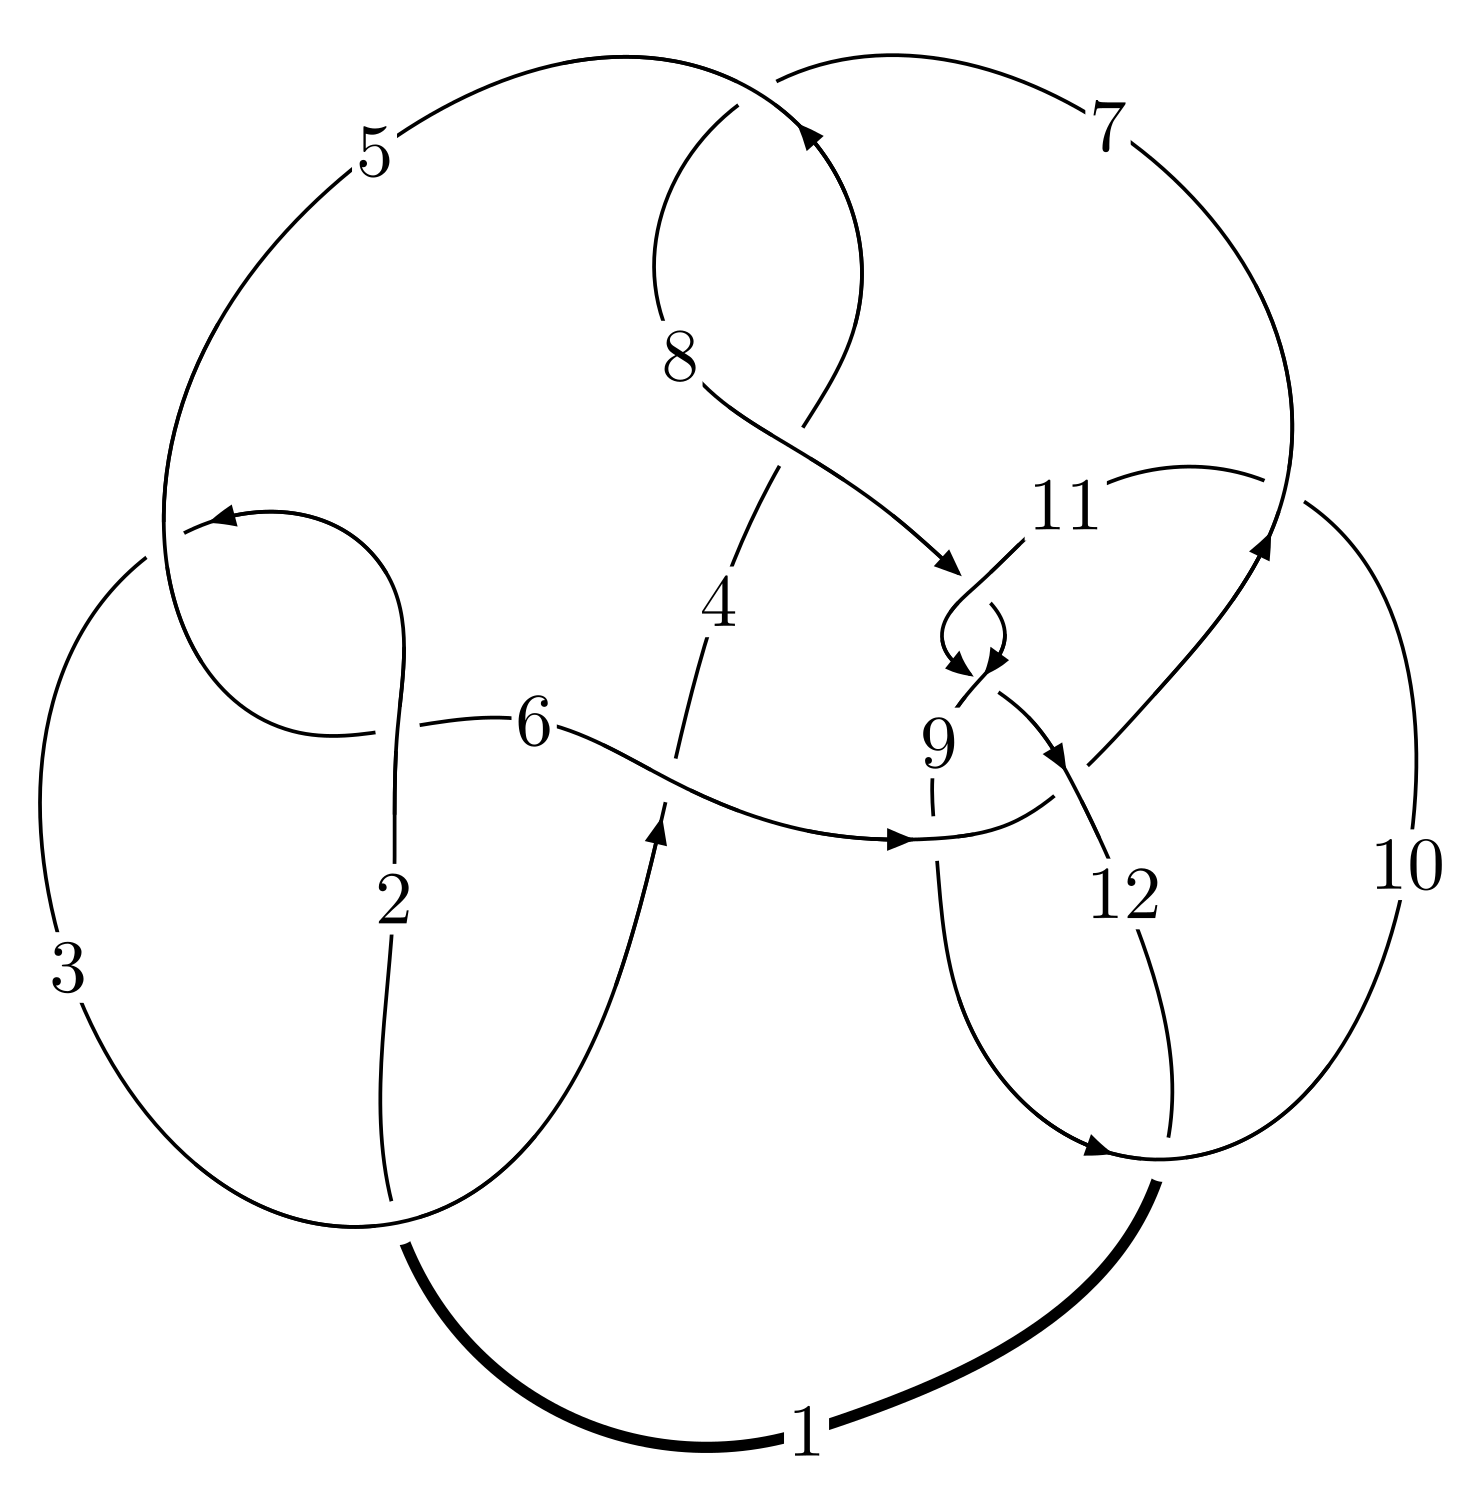
\includegraphics[width=112pt]{../../../GIT/diagram.site/Diagrams/png/2110_12n_0021.png}\\
\ \ \ A knot diagram\footnotemark}&
\allowdisplaybreaks
\textbf{Linearized knot diagam} \\
\cline{2-2}
 &
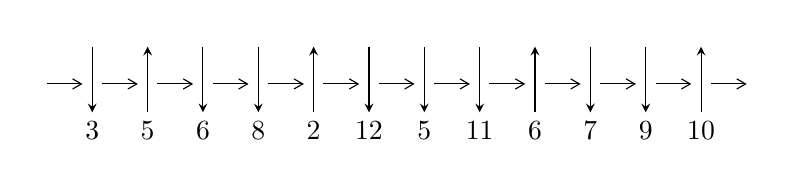
\begin{tikzpicture}[x=20pt, y=17pt]
	% nodes
	\node (C0) at (0, 0) {};
	\node (C1) at (1, 0) {};
	\node (C1U) at (1, +1) {};
	\node (C1D) at (1, -1) {3};

	\node (C2) at (2, 0) {};
	\node (C2U) at (2, +1) {};
	\node (C2D) at (2, -1) {5};

	\node (C3) at (3, 0) {};
	\node (C3U) at (3, +1) {};
	\node (C3D) at (3, -1) {6};

	\node (C4) at (4, 0) {};
	\node (C4U) at (4, +1) {};
	\node (C4D) at (4, -1) {8};

	\node (C5) at (5, 0) {};
	\node (C5U) at (5, +1) {};
	\node (C5D) at (5, -1) {2};

	\node (C6) at (6, 0) {};
	\node (C6U) at (6, +1) {};
	\node (C6D) at (6, -1) {12};

	\node (C7) at (7, 0) {};
	\node (C7U) at (7, +1) {};
	\node (C7D) at (7, -1) {5};

	\node (C8) at (8, 0) {};
	\node (C8U) at (8, +1) {};
	\node (C8D) at (8, -1) {11};

	\node (C9) at (9, 0) {};
	\node (C9U) at (9, +1) {};
	\node (C9D) at (9, -1) {6};

	\node (C10) at (10, 0) {};
	\node (C10U) at (10, +1) {};
	\node (C10D) at (10, -1) {7};

	\node (C11) at (11, 0) {};
	\node (C11U) at (11, +1) {};
	\node (C11D) at (11, -1) {9};

	\node (C12) at (12, 0) {};
	\node (C12U) at (12, +1) {};
	\node (C12D) at (12, -1) {10};
	\node (C13) at (13, 0) {};

	% arrows
	\draw[->,>={angle 60}]
	(C0) edge (C1) (C1) edge (C2) (C2) edge (C3) (C3) edge (C4) (C4) edge (C5) (C5) edge (C6) (C6) edge (C7) (C7) edge (C8) (C8) edge (C9) (C9) edge (C10) (C10) edge (C11) (C11) edge (C12) (C12) edge (C13) ;	\draw[->,>=stealth]
	(C1U) edge (C1D) (C2D) edge (C2U) (C3U) edge (C3D) (C4U) edge (C4D) (C5D) edge (C5U) (C6U) edge (C6D) (C7U) edge (C7D) (C8U) edge (C8D) (C9D) edge (C9U) (C10U) edge (C10D) (C11U) edge (C11D) (C12D) edge (C12U) ;
	\end{tikzpicture} \\
\hhline{~~} \\& 
\textbf{Solving Sequence} \\ \cline{2-2} 
 &
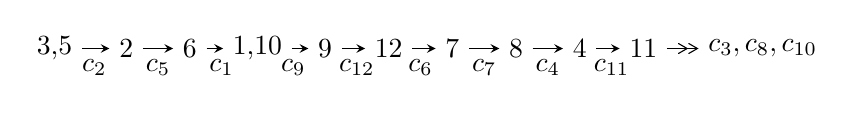
\begin{tikzpicture}[x=23pt, y=7pt]
	% node
	\node (A0) at (-1/8, 0) {3,5};
	\node (A1) at (1, 0) {2};
	\node (A2) at (2, 0) {6};
	\node (A3) at (49/16, 0) {1,10};
	\node (A4) at (33/8, 0) {9};
	\node (A5) at (41/8, 0) {12};
	\node (A6) at (49/8, 0) {7};
	\node (A7) at (57/8, 0) {8};
	\node (A8) at (65/8, 0) {4};
	\node (A9) at (73/8, 0) {11};
	\node (C1) at (1/2, -1) {$c_{2}$};
	\node (C2) at (3/2, -1) {$c_{5}$};
	\node (C3) at (5/2, -1) {$c_{1}$};
	\node (C4) at (29/8, -1) {$c_{9}$};
	\node (C5) at (37/8, -1) {$c_{12}$};
	\node (C6) at (45/8, -1) {$c_{6}$};
	\node (C7) at (53/8, -1) {$c_{7}$};
	\node (C8) at (61/8, -1) {$c_{4}$};
	\node (C9) at (69/8, -1) {$c_{11}$};
	\node (A10) at (11, 0) {$c_{3},c_{8},c_{10}$};

	% edge
	\draw[->,>=stealth]	
	(A0) edge (A1) (A1) edge (A2) (A2) edge (A3) (A3) edge (A4) (A4) edge (A5) (A5) edge (A6) (A6) edge (A7) (A7) edge (A8) (A8) edge (A9) ;
	\draw[->>,>={angle 60}]	
	(A9) edge (A10);
\end{tikzpicture} \\ 

\end{tabular} \\

\footnotetext{
The image of knot diagram is generated by the software ``\textbf{Draw programme}" developed by Andrew Bartholomew(\url{http://www.layer8.co.uk/maths/draw/index.htm\#Running-draw}), where we modified some parts for our purpose(\url{https://github.com/CATsTAILs/LinksPainter}).
}\phantom \\ \newline 
\centering \textbf{Ideals for irreducible components\footnotemark of $X_{\text{par}}$} 
 
\begin{align*}
I^u_{1}&=\langle 
-1.31031\times10^{60} u^{73}+8.78516\times10^{60} u^{72}+\cdots+8.05327\times10^{59} b+2.46563\times10^{59},\\
\phantom{I^u_{1}}&\phantom{= \langle  }-1.87533\times10^{60} u^{73}+1.24710\times10^{61} u^{72}+\cdots+8.05327\times10^{59} a-7.86574\times10^{60},\\
\phantom{I^u_{1}}&\phantom{= \langle  }u^{74}-7 u^{73}+\cdots-10 u+1\rangle \\
I^u_{2}&=\langle 
-2 a^4 u+9 a^3 u+9 a^3-10 a^2-6 a u+5 b+4 u+4,\;a^5+5 a^4 u-6 a^3 u-6 a^3+3 a^2+a u- u-1,\;u^2+u+1\rangle \\
I^u_{3}&=\langle 
-2 u^4+2 u^3-2 u^2+b- u+2,\;- u^4+3 u^3-4 u^2+a+4 u-1,\;u^5- u^4+2 u^3- u^2+u-1\rangle \\
\\
\end{align*}
\raggedright * 3 irreducible components of $\dim_{\mathbb{C}}=0$, with total 89 representations.\\
\footnotetext{All coefficients of polynomials are rational numbers. But the coefficients are sometimes approximated in decimal forms when there is not enough margin.}
\newpage
\renewcommand{\arraystretch}{1}
\centering \section*{I. $I^u_{1}= \langle -1.31\times10^{60} u^{73}+8.79\times10^{60} u^{72}+\cdots+8.05\times10^{59} b+2.47\times10^{59},\;-1.88\times10^{60} u^{73}+1.25\times10^{61} u^{72}+\cdots+8.05\times10^{59} a-7.87\times10^{60},\;u^{74}-7 u^{73}+\cdots-10 u+1 \rangle$}
\flushleft \textbf{(i) Arc colorings}\\
\begin{tabular}{m{7pt} m{180pt} m{7pt} m{180pt} }
\flushright $a_{3}=$&$\begin{pmatrix}1\\0\end{pmatrix}$ \\
\flushright $a_{5}=$&$\begin{pmatrix}0\\u\end{pmatrix}$ \\
\flushright $a_{2}=$&$\begin{pmatrix}1\\u^2\end{pmatrix}$ \\
\flushright $a_{6}=$&$\begin{pmatrix}u\\u^3+u\end{pmatrix}$ \\
\flushright $a_{1}=$&$\begin{pmatrix}u^2+1\\u^2\end{pmatrix}$ \\
\flushright $a_{10}=$&$\begin{pmatrix}2.32865 u^{73}-15.4857 u^{72}+\cdots+29.2596 u+9.76713\\1.62705 u^{73}-10.9088 u^{72}+\cdots-4.88417 u-0.306165\end{pmatrix}$ \\
\flushright $a_{9}=$&$\begin{pmatrix}1.30294 u^{73}-8.68046 u^{72}+\cdots+15.6245 u+11.1275\\0.928079 u^{73}-4.66399 u^{72}+\cdots-21.2414 u+1.42898\end{pmatrix}$ \\
\flushright $a_{12}=$&$\begin{pmatrix}0.0128426 u^{73}-0.606575 u^{72}+\cdots-24.6025 u-4.47929\\-1.07283 u^{73}+7.86599 u^{72}+\cdots-13.6469 u+1.79816\end{pmatrix}$ \\
\flushright $a_{7}=$&$\begin{pmatrix}-1.84067 u^{73}+11.0360 u^{72}+\cdots-8.87375 u-2.84119\\-1.31744 u^{73}+10.0636 u^{72}+\cdots-16.1390 u+2.16705\end{pmatrix}$ \\
\flushright $a_{8}=$&$\begin{pmatrix}-1.84067 u^{73}+11.0360 u^{72}+\cdots-8.87375 u-2.84119\\-1.23075 u^{73}+11.7949 u^{72}+\cdots-32.7857 u+4.01579\end{pmatrix}$ \\
\flushright $a_{4}=$&$\begin{pmatrix}u^4+u^2+1\\u^6+2 u^4+u^2\end{pmatrix}$ \\
\flushright $a_{11}=$&$\begin{pmatrix}0.612092 u^{73}-4.77433 u^{72}+\cdots+2.25396 u+7.51995\\-0.187474 u^{73}+4.35220 u^{72}+\cdots-38.3916 u+3.65569\end{pmatrix}$\\&\end{tabular}
\flushleft \textbf{(ii) Obstruction class $= -1$}\\~\\
\flushleft \textbf{(iii) Cusp Shapes $= -12.9104 u^{73}+92.7725 u^{72}+\cdots-82.6450 u+3.33954$}\\~\\
\newpage\renewcommand{\arraystretch}{1}
\flushleft \textbf{(iv) u-Polynomials at the component}\newline \\
\begin{tabular}{m{50pt}|m{274pt}}
Crossings & \hspace{64pt}u-Polynomials at each crossing \\
\hline $$\begin{aligned}c_{1}\end{aligned}$$&$\begin{aligned}
&u^{74}+23 u^{73}+\cdots-168 u+1
\end{aligned}$\\
\hline $$\begin{aligned}c_{2},c_{5}\end{aligned}$$&$\begin{aligned}
&u^{74}+7 u^{73}+\cdots+10 u+1
\end{aligned}$\\
\hline $$\begin{aligned}c_{3}\end{aligned}$$&$\begin{aligned}
&u^{74}-7 u^{73}+\cdots+23935148 u+1174793
\end{aligned}$\\
\hline $$\begin{aligned}c_{4},c_{7}\end{aligned}$$&$\begin{aligned}
&u^{74}-2 u^{73}+\cdots+3072 u+1024
\end{aligned}$\\
\hline $$\begin{aligned}c_{6}\end{aligned}$$&$\begin{aligned}
&u^{74}-4 u^{73}+\cdots+3 u-1
\end{aligned}$\\
\hline $$\begin{aligned}c_{8},c_{11}\end{aligned}$$&$\begin{aligned}
&u^{74}-8 u^{73}+\cdots-83 u-1
\end{aligned}$\\
\hline $$\begin{aligned}c_{9}\end{aligned}$$&$\begin{aligned}
&u^{74}-4 u^{73}+\cdots+18563 u+7979
\end{aligned}$\\
\hline $$\begin{aligned}c_{10}\end{aligned}$$&$\begin{aligned}
&u^{74}+2 u^{73}+\cdots+140788 u-6632
\end{aligned}$\\
\hline $$\begin{aligned}c_{12}\end{aligned}$$&$\begin{aligned}
&u^{74}+11 u^{73}+\cdots+600 u^2+32
\end{aligned}$\\
\hline
\end{tabular}\\~\\
\newpage\renewcommand{\arraystretch}{1}
\flushleft \textbf{(v) Riley Polynomials at the component}\newline \\
\begin{tabular}{m{50pt}|m{274pt}}
Crossings & \hspace{64pt}Riley Polynomials at each crossing \\
\hline $$\begin{aligned}c_{1}\end{aligned}$$&$\begin{aligned}
&y^{74}+63 y^{73}+\cdots-33884 y+1
\end{aligned}$\\
\hline $$\begin{aligned}c_{2},c_{5}\end{aligned}$$&$\begin{aligned}
&y^{74}+23 y^{73}+\cdots-168 y+1
\end{aligned}$\\
\hline $$\begin{aligned}c_{3}\end{aligned}$$&$\begin{aligned}
&y^{74}+103 y^{73}+\cdots-195612233228368 y+1380138592849
\end{aligned}$\\
\hline $$\begin{aligned}c_{4},c_{7}\end{aligned}$$&$\begin{aligned}
&y^{74}+50 y^{73}+\cdots+5242880 y+1048576
\end{aligned}$\\
\hline $$\begin{aligned}c_{6}\end{aligned}$$&$\begin{aligned}
&y^{74}-20 y^{73}+\cdots+y+1
\end{aligned}$\\
\hline $$\begin{aligned}c_{8},c_{11}\end{aligned}$$&$\begin{aligned}
&y^{74}-40 y^{73}+\cdots-2497 y+1
\end{aligned}$\\
\hline $$\begin{aligned}c_{9}\end{aligned}$$&$\begin{aligned}
&y^{74}+46 y^{73}+\cdots-1411728345 y+63664441
\end{aligned}$\\
\hline $$\begin{aligned}c_{10}\end{aligned}$$&$\begin{aligned}
&y^{74}+78 y^{73}+\cdots-8817552656 y+43983424
\end{aligned}$\\
\hline $$\begin{aligned}c_{12}\end{aligned}$$&$\begin{aligned}
&y^{74}-27 y^{73}+\cdots+38400 y+1024
\end{aligned}$\\
\hline
\end{tabular}\\~\\
\newpage\flushleft \textbf{(vi) Complex Volumes and Cusp Shapes}
$$\begin{array}{c|c|c}  
\text{Solutions to }I^u_{1}& \I (\text{vol} + \sqrt{-1}CS) & \text{Cusp shape}\\
 \hline 
\begin{aligned}
u &= -0.588568 + 0.781606 I \\
a &= \phantom{-}2.11655 - 1.27106 I \\
b &= -0.34086 - 1.74865 I\end{aligned}
 & -0.94329 - 1.13464 I & \phantom{-0.000000 } 0 \\ \hline\begin{aligned}
u &= -0.588568 - 0.781606 I \\
a &= \phantom{-}2.11655 + 1.27106 I \\
b &= -0.34086 + 1.74865 I\end{aligned}
 & -0.94329 + 1.13464 I & \phantom{-0.000000 } 0 \\ \hline\begin{aligned}
u &= -0.224608 + 0.939787 I \\
a &= -1.43760 - 1.52815 I \\
b &= -1.80851 + 0.25423 I\end{aligned}
 & -3.42601 - 3.36523 I & \phantom{-0.000000 } 0 \\ \hline\begin{aligned}
u &= -0.224608 - 0.939787 I \\
a &= -1.43760 + 1.52815 I \\
b &= -1.80851 - 0.25423 I\end{aligned}
 & -3.42601 + 3.36523 I & \phantom{-0.000000 } 0 \\ \hline\begin{aligned}
u &= -0.480747 + 0.917533 I \\
a &= \phantom{-}3.51191 - 3.12500 I \\
b &= -1.37679 - 5.49401 I\end{aligned}
 & -2.18804 - 1.82733 I & \phantom{-0.000000 } 0 \\ \hline\begin{aligned}
u &= -0.480747 - 0.917533 I \\
a &= \phantom{-}3.51191 + 3.12500 I \\
b &= -1.37679 + 5.49401 I\end{aligned}
 & -2.18804 + 1.82733 I & \phantom{-0.000000 } 0 \\ \hline\begin{aligned}
u &= -0.948295 + 0.114817 I \\
a &= \phantom{-}0.642760 - 0.299680 I \\
b &= -0.384036 - 0.001201 I\end{aligned}
 & \phantom{-}2.84481 - 6.06997 I & \phantom{-0.000000 -}0. + 5.46750 I \\ \hline\begin{aligned}
u &= -0.948295 - 0.114817 I \\
a &= \phantom{-}0.642760 + 0.299680 I \\
b &= -0.384036 + 0.001201 I\end{aligned}
 & \phantom{-}2.84481 + 6.06997 I & \phantom{-0.000000 } 0. - 5.46750 I \\ \hline\begin{aligned}
u &= -0.605694 + 0.882842 I \\
a &= \phantom{-}1.04425 - 1.21226 I \\
b &= \phantom{-}0.30514 - 2.02629 I\end{aligned}
 & -1.25518 - 3.58366 I & \phantom{-0.000000 } 0 \\ \hline\begin{aligned}
u &= -0.605694 - 0.882842 I \\
a &= \phantom{-}1.04425 + 1.21226 I \\
b &= \phantom{-}0.30514 + 2.02629 I\end{aligned}
 & -1.25518 + 3.58366 I & \phantom{-0.000000 } 0\\
 \hline 
 \end{array}$$\newpage$$\begin{array}{c|c|c}  
\text{Solutions to }I^u_{1}& \I (\text{vol} + \sqrt{-1}CS) & \text{Cusp shape}\\
 \hline 
\begin{aligned}
u &= -0.363037 + 0.817565 I \\
a &= \phantom{-}0.599509 - 0.288116 I \\
b &= -0.309360 - 0.528307 I\end{aligned}
 & -0.31180 - 1.54577 I & -2.35841 + 4.98495 I \\ \hline\begin{aligned}
u &= -0.363037 - 0.817565 I \\
a &= \phantom{-}0.599509 + 0.288116 I \\
b &= -0.309360 + 0.528307 I\end{aligned}
 & -0.31180 + 1.54577 I & -2.35841 - 4.98495 I \\ \hline\begin{aligned}
u &= \phantom{-}0.377437 + 0.795068 I \\
a &= \phantom{-}0.458626 - 0.671697 I \\
b &= -0.886331 - 0.076122 I\end{aligned}
 & -6.11124 + 6.05756 I & -13.16929 + 2.49659 I \\ \hline\begin{aligned}
u &= \phantom{-}0.377437 - 0.795068 I \\
a &= \phantom{-}0.458626 + 0.671697 I \\
b &= -0.886331 + 0.076122 I\end{aligned}
 & -6.11124 - 6.05756 I & -13.16929 - 2.49659 I \\ \hline\begin{aligned}
u &= \phantom{-}0.879036\phantom{ +0.000000I} \\
a &= \phantom{-}0.464133\phantom{ +0.000000I} \\
b &= -0.0979340\phantom{ +0.000000I}\end{aligned}
 & -3.60099\phantom{ +0.000000I} & \phantom{-}6.20630\phantom{ +0.000000I} \\ \hline\begin{aligned}
u &= \phantom{-}0.424038 + 0.768258 I \\
a &= -0.668714 + 0.128685 I \\
b &= \phantom{-}0.451674 + 0.637183 I\end{aligned}
 & -5.95413 - 2.77149 I & -11.1970 + 11.7984 I \\ \hline\begin{aligned}
u &= \phantom{-}0.424038 - 0.768258 I \\
a &= -0.668714 - 0.128685 I \\
b &= \phantom{-}0.451674 - 0.637183 I\end{aligned}
 & -5.95413 + 2.77149 I & -11.1970 - 11.7984 I \\ \hline\begin{aligned}
u &= -0.789645 + 0.824107 I \\
a &= -0.35319 + 1.72243 I \\
b &= \phantom{-}1.27854 + 1.76922 I\end{aligned}
 & \phantom{-}3.57080 - 3.55900 I & \phantom{-0.000000 } 0 \\ \hline\begin{aligned}
u &= -0.789645 - 0.824107 I \\
a &= -0.35319 - 1.72243 I \\
b &= \phantom{-}1.27854 - 1.76922 I\end{aligned}
 & \phantom{-}3.57080 + 3.55900 I & \phantom{-0.000000 } 0 \\ \hline\begin{aligned}
u &= \phantom{-}0.926734 + 0.675434 I \\
a &= -0.503809 - 1.111700 I \\
b &= \phantom{-}0.37933 - 1.50865 I\end{aligned}
 & \phantom{-}7.41718 - 3.39847 I & \phantom{-0.000000 } 0\\
 \hline 
 \end{array}$$\newpage$$\begin{array}{c|c|c}  
\text{Solutions to }I^u_{1}& \I (\text{vol} + \sqrt{-1}CS) & \text{Cusp shape}\\
 \hline 
\begin{aligned}
u &= \phantom{-}0.926734 - 0.675434 I \\
a &= -0.503809 + 1.111700 I \\
b &= \phantom{-}0.37933 + 1.50865 I\end{aligned}
 & \phantom{-}7.41718 + 3.39847 I & \phantom{-0.000000 } 0 \\ \hline\begin{aligned}
u &= -0.357389 + 1.093680 I \\
a &= \phantom{-}0.227043 - 0.773438 I \\
b &= -0.030211 + 0.326577 I\end{aligned}
 & \phantom{-}0.97521 - 4.62256 I & \phantom{-0.000000 } 0 \\ \hline\begin{aligned}
u &= -0.357389 - 1.093680 I \\
a &= \phantom{-}0.227043 + 0.773438 I \\
b &= -0.030211 - 0.326577 I\end{aligned}
 & \phantom{-}0.97521 + 4.62256 I & \phantom{-0.000000 } 0 \\ \hline\begin{aligned}
u &= \phantom{-}0.820006 + 0.826808 I \\
a &= \phantom{-}0.158463 + 0.704129 I \\
b &= -1.384830 + 0.014374 I\end{aligned}
 & \phantom{-}3.14985 - 1.37670 I & \phantom{-0.000000 } 0 \\ \hline\begin{aligned}
u &= \phantom{-}0.820006 - 0.826808 I \\
a &= \phantom{-}0.158463 - 0.704129 I \\
b &= -1.384830 - 0.014374 I\end{aligned}
 & \phantom{-}3.14985 + 1.37670 I & \phantom{-0.000000 } 0 \\ \hline\begin{aligned}
u &= -0.168266 + 1.155270 I \\
a &= \phantom{-}0.511207 - 0.231030 I \\
b &= -0.109347 + 0.212969 I\end{aligned}
 & -0.18048 - 2.67430 I & \phantom{-0.000000 } 0 \\ \hline\begin{aligned}
u &= -0.168266 - 1.155270 I \\
a &= \phantom{-}0.511207 + 0.231030 I \\
b &= -0.109347 - 0.212969 I\end{aligned}
 & -0.18048 + 2.67430 I & \phantom{-0.000000 } 0 \\ \hline\begin{aligned}
u &= -0.315143 + 0.768424 I \\
a &= -1.52568 + 6.21959 I \\
b &= \phantom{-}6.24699 + 1.55706 I\end{aligned}
 & -1.96434 - 1.46942 I & \phantom{-}69.4609 - 82.1819 I \\ \hline\begin{aligned}
u &= -0.315143 - 0.768424 I \\
a &= -1.52568 - 6.21959 I \\
b &= \phantom{-}6.24699 - 1.55706 I\end{aligned}
 & -1.96434 + 1.46942 I & \phantom{-}69.4609 + 82.1819 I \\ \hline\begin{aligned}
u &= -0.817564 + 0.115016 I \\
a &= -0.102494 - 0.097733 I \\
b &= \phantom{-}0.693608 + 0.178324 I\end{aligned}
 & \phantom{-}4.23425 + 0.54410 I & \phantom{-}1.60258 - 0.06952 I\\
 \hline 
 \end{array}$$\newpage$$\begin{array}{c|c|c}  
\text{Solutions to }I^u_{1}& \I (\text{vol} + \sqrt{-1}CS) & \text{Cusp shape}\\
 \hline 
\begin{aligned}
u &= -0.817564 - 0.115016 I \\
a &= -0.102494 + 0.097733 I \\
b &= \phantom{-}0.693608 - 0.178324 I\end{aligned}
 & \phantom{-}4.23425 - 0.54410 I & \phantom{-}1.60258 + 0.06952 I \\ \hline\begin{aligned}
u &= \phantom{-}0.782206 + 0.888648 I \\
a &= \phantom{-}1.29280 + 1.39998 I \\
b &= -0.63121 + 2.77026 I\end{aligned}
 & \phantom{-}1.01094 + 2.94591 I & \phantom{-0.000000 } 0 \\ \hline\begin{aligned}
u &= \phantom{-}0.782206 - 0.888648 I \\
a &= \phantom{-}1.29280 - 1.39998 I \\
b &= -0.63121 - 2.77026 I\end{aligned}
 & \phantom{-}1.01094 - 2.94591 I & \phantom{-0.000000 } 0 \\ \hline\begin{aligned}
u &= \phantom{-}0.960126 + 0.695377 I \\
a &= \phantom{-}1.22788 + 1.52034 I \\
b &= \phantom{-}0.01982 + 2.23698 I\end{aligned}
 & \phantom{-}6.50731 - 10.89880 I & \phantom{-0.000000 } 0 \\ \hline\begin{aligned}
u &= \phantom{-}0.960126 - 0.695377 I \\
a &= \phantom{-}1.22788 - 1.52034 I \\
b &= \phantom{-}0.01982 - 2.23698 I\end{aligned}
 & \phantom{-}6.50731 + 10.89880 I & \phantom{-0.000000 } 0 \\ \hline\begin{aligned}
u &= -0.099605 + 0.797661 I \\
a &= -1.28212 + 0.66262 I \\
b &= -0.983447 + 0.821591 I\end{aligned}
 & -3.94950 - 0.19450 I & -14.2244 + 0.5338 I \\ \hline\begin{aligned}
u &= -0.099605 - 0.797661 I \\
a &= -1.28212 - 0.66262 I \\
b &= -0.983447 - 0.821591 I\end{aligned}
 & -3.94950 + 0.19450 I & -14.2244 - 0.5338 I \\ \hline\begin{aligned}
u &= \phantom{-}0.913271 + 0.785754 I \\
a &= -1.24292 - 1.30749 I \\
b &= -0.04215 - 2.39793 I\end{aligned}
 & \phantom{-}9.56303 - 3.64207 I & \phantom{-0.000000 } 0 \\ \hline\begin{aligned}
u &= \phantom{-}0.913271 - 0.785754 I \\
a &= -1.24292 + 1.30749 I \\
b &= -0.04215 + 2.39793 I\end{aligned}
 & \phantom{-}9.56303 + 3.64207 I & \phantom{-0.000000 } 0 \\ \hline\begin{aligned}
u &= \phantom{-}0.837187 + 0.871109 I \\
a &= -2.00342 + 0.20473 I \\
b &= -0.960890 - 0.793882 I\end{aligned}
 & \phantom{-}4.88888 + 2.03616 I & \phantom{-0.000000 } 0\\
 \hline 
 \end{array}$$\newpage$$\begin{array}{c|c|c}  
\text{Solutions to }I^u_{1}& \I (\text{vol} + \sqrt{-1}CS) & \text{Cusp shape}\\
 \hline 
\begin{aligned}
u &= \phantom{-}0.837187 - 0.871109 I \\
a &= -2.00342 - 0.20473 I \\
b &= -0.960890 + 0.793882 I\end{aligned}
 & \phantom{-}4.88888 - 2.03616 I & \phantom{-0.000000 } 0 \\ \hline\begin{aligned}
u &= -0.753364 + 0.950514 I \\
a &= -1.37943 + 0.51575 I \\
b &= -0.46215 + 1.85324 I\end{aligned}
 & \phantom{-}3.17540 - 2.27063 I & \phantom{-0.000000 } 0 \\ \hline\begin{aligned}
u &= -0.753364 - 0.950514 I \\
a &= -1.37943 - 0.51575 I \\
b &= -0.46215 - 1.85324 I\end{aligned}
 & \phantom{-}3.17540 + 2.27063 I & \phantom{-0.000000 } 0 \\ \hline\begin{aligned}
u &= -0.883272 + 0.834733 I \\
a &= \phantom{-}1.35545 - 1.08459 I \\
b &= \phantom{-}0.24804 - 1.97325 I\end{aligned}
 & \phantom{-}2.10183 + 2.80934 I & \phantom{-0.000000 } 0 \\ \hline\begin{aligned}
u &= -0.883272 - 0.834733 I \\
a &= \phantom{-}1.35545 + 1.08459 I \\
b &= \phantom{-}0.24804 + 1.97325 I\end{aligned}
 & \phantom{-}2.10183 - 2.80934 I & \phantom{-0.000000 } 0 \\ \hline\begin{aligned}
u &= \phantom{-}0.784779 + 0.950831 I \\
a &= \phantom{-}0.418763 - 0.127905 I \\
b &= \phantom{-}1.32211 + 1.05195 I\end{aligned}
 & \phantom{-}2.76643 + 7.39057 I & \phantom{-0.000000 } 0 \\ \hline\begin{aligned}
u &= \phantom{-}0.784779 - 0.950831 I \\
a &= \phantom{-}0.418763 + 0.127905 I \\
b &= \phantom{-}1.32211 - 1.05195 I\end{aligned}
 & \phantom{-}2.76643 - 7.39057 I & \phantom{-0.000000 } 0 \\ \hline\begin{aligned}
u &= \phantom{-}0.817309 + 0.927924 I \\
a &= \phantom{-}0.88430 - 1.76207 I \\
b &= \phantom{-}1.34165 - 1.29399 I\end{aligned}
 & \phantom{-}4.71109 + 4.13291 I & \phantom{-0.000000 } 0 \\ \hline\begin{aligned}
u &= \phantom{-}0.817309 - 0.927924 I \\
a &= \phantom{-}0.88430 + 1.76207 I \\
b &= \phantom{-}1.34165 + 1.29399 I\end{aligned}
 & \phantom{-}4.71109 - 4.13291 I & \phantom{-0.000000 } 0 \\ \hline\begin{aligned}
u &= -0.251345 + 1.227450 I \\
a &= -0.570312 + 0.368260 I \\
b &= -0.543530 - 0.574793 I\end{aligned}
 & -1.87183 - 10.09290 I & \phantom{-0.000000 } 0\\
 \hline 
 \end{array}$$\newpage$$\begin{array}{c|c|c}  
\text{Solutions to }I^u_{1}& \I (\text{vol} + \sqrt{-1}CS) & \text{Cusp shape}\\
 \hline 
\begin{aligned}
u &= -0.251345 - 1.227450 I \\
a &= -0.570312 - 0.368260 I \\
b &= -0.543530 + 0.574793 I\end{aligned}
 & -1.87183 + 10.09290 I & \phantom{-0.000000 } 0 \\ \hline\begin{aligned}
u &= \phantom{-}0.943453 + 0.828089 I \\
a &= \phantom{-}0.60572 + 1.39990 I \\
b &= -0.38320 + 1.76670 I\end{aligned}
 & \phantom{-}9.18515 + 2.01287 I & \phantom{-0.000000 } 0 \\ \hline\begin{aligned}
u &= \phantom{-}0.943453 - 0.828089 I \\
a &= \phantom{-}0.60572 - 1.39990 I \\
b &= -0.38320 - 1.76670 I\end{aligned}
 & \phantom{-}9.18515 - 2.01287 I & \phantom{-0.000000 } 0 \\ \hline\begin{aligned}
u &= -0.826585 + 0.970325 I \\
a &= \phantom{-}0.76341 - 1.66069 I \\
b &= -0.86711 - 2.14556 I\end{aligned}
 & \phantom{-}1.67555 - 9.13934 I & \phantom{-0.000000 } 0 \\ \hline\begin{aligned}
u &= -0.826585 - 0.970325 I \\
a &= \phantom{-}0.76341 + 1.66069 I \\
b &= -0.86711 + 2.14556 I\end{aligned}
 & \phantom{-}1.67555 + 9.13934 I & \phantom{-0.000000 } 0 \\ \hline\begin{aligned}
u &= -0.419590 + 1.216660 I \\
a &= -0.286830 - 0.137018 I \\
b &= \phantom{-}0.092382 - 0.684597 I\end{aligned}
 & -0.83764 + 1.21344 I & \phantom{-0.000000 } 0 \\ \hline\begin{aligned}
u &= -0.419590 - 1.216660 I \\
a &= -0.286830 + 0.137018 I \\
b &= \phantom{-}0.092382 + 0.684597 I\end{aligned}
 & -0.83764 - 1.21344 I & \phantom{-0.000000 } 0 \\ \hline\begin{aligned}
u &= \phantom{-}0.432353 + 1.221260 I \\
a &= -0.162125 - 0.020944 I \\
b &= -0.245061 + 0.213540 I\end{aligned}
 & -7.41606 + 4.57419 I & \phantom{-0.000000 } 0 \\ \hline\begin{aligned}
u &= \phantom{-}0.432353 - 1.221260 I \\
a &= -0.162125 + 0.020944 I \\
b &= -0.245061 - 0.213540 I\end{aligned}
 & -7.41606 - 4.57419 I & \phantom{-0.000000 } 0 \\ \hline\begin{aligned}
u &= \phantom{-}0.814545 + 1.015150 I \\
a &= -1.14539 - 1.49821 I \\
b &= \phantom{-}0.80502 - 2.49598 I\end{aligned}
 & \phantom{-}8.83947 + 10.02070 I & \phantom{-0.000000 } 0\\
 \hline 
 \end{array}$$\newpage$$\begin{array}{c|c|c}  
\text{Solutions to }I^u_{1}& \I (\text{vol} + \sqrt{-1}CS) & \text{Cusp shape}\\
 \hline 
\begin{aligned}
u &= \phantom{-}0.814545 - 1.015150 I \\
a &= -1.14539 + 1.49821 I \\
b &= \phantom{-}0.80502 + 2.49598 I\end{aligned}
 & \phantom{-}8.83947 - 10.02070 I & \phantom{-0.000000 } 0 \\ \hline\begin{aligned}
u &= \phantom{-}0.764489 + 1.073570 I \\
a &= -0.940897 - 0.743631 I \\
b &= \phantom{-}0.18830 - 1.69305 I\end{aligned}
 & \phantom{-}6.17331 + 9.63827 I & \phantom{-0.000000 } 0 \\ \hline\begin{aligned}
u &= \phantom{-}0.764489 - 1.073570 I \\
a &= -0.940897 + 0.743631 I \\
b &= \phantom{-}0.18830 + 1.69305 I\end{aligned}
 & \phantom{-}6.17331 - 9.63827 I & \phantom{-0.000000 } 0 \\ \hline\begin{aligned}
u &= \phantom{-}0.853280 + 1.005800 I \\
a &= \phantom{-}1.16762 + 1.03945 I \\
b &= -0.02363 + 1.82898 I\end{aligned}
 & \phantom{-}8.61435 + 4.58115 I & \phantom{-0.000000 } 0 \\ \hline\begin{aligned}
u &= \phantom{-}0.853280 - 1.005800 I \\
a &= \phantom{-}1.16762 - 1.03945 I \\
b &= -0.02363 - 1.82898 I\end{aligned}
 & \phantom{-}8.61435 - 4.58115 I & \phantom{-0.000000 } 0 \\ \hline\begin{aligned}
u &= \phantom{-}0.787160 + 1.077840 I \\
a &= \phantom{-}1.21504 + 1.50799 I \\
b &= -0.57962 + 2.58206 I\end{aligned}
 & \phantom{-}5.3004 + 17.3091 I & \phantom{-0.000000 } 0 \\ \hline\begin{aligned}
u &= \phantom{-}0.787160 - 1.077840 I \\
a &= \phantom{-}1.21504 - 1.50799 I \\
b &= -0.57962 - 2.58206 I\end{aligned}
 & \phantom{-}5.3004 - 17.3091 I & \phantom{-0.000000 } 0 \\ \hline\begin{aligned}
u &= \phantom{-}0.093711 + 0.582935 I \\
a &= -0.60542 + 1.79370 I \\
b &= \phantom{-}0.945378 + 0.484928 I\end{aligned}
 & -0.76340 + 2.05732 I & -6.61172 - 3.28073 I \\ \hline\begin{aligned}
u &= \phantom{-}0.093711 - 0.582935 I \\
a &= -0.60542 - 1.79370 I \\
b &= \phantom{-}0.945378 - 0.484928 I\end{aligned}
 & -0.76340 - 2.05732 I & -6.61172 + 3.28073 I \\ \hline\begin{aligned}
u &= -0.116761 + 0.531053 I \\
a &= \phantom{-}1.61823 - 1.25855 I \\
b &= -0.582250 - 0.676718 I\end{aligned}
 & -0.75534 - 1.25758 I & -6.16688 + 4.20297 I\\
 \hline 
 \end{array}$$\newpage$$\begin{array}{c|c|c}  
\text{Solutions to }I^u_{1}& \I (\text{vol} + \sqrt{-1}CS) & \text{Cusp shape}\\
 \hline 
\begin{aligned}
u &= -0.116761 - 0.531053 I \\
a &= \phantom{-}1.61823 + 1.25855 I \\
b &= -0.582250 + 0.676718 I\end{aligned}
 & -0.75534 + 1.25758 I & -6.16688 - 4.20297 I \\ \hline\begin{aligned}
u &= -0.298970 + 0.158249 I \\
a &= \phantom{-}2.38582 - 3.03610 I \\
b &= -0.052906 - 1.134690 I\end{aligned}
 & -0.71671 - 1.37236 I & -4.04860 + 4.25236 I \\ \hline\begin{aligned}
u &= -0.298970 - 0.158249 I \\
a &= \phantom{-}2.38582 + 3.03610 I \\
b &= -0.052906 + 1.134690 I\end{aligned}
 & -0.71671 + 1.37236 I & -4.04860 - 4.25236 I \\ \hline\begin{aligned}
u &= \phantom{-}0.0736878\phantom{ +0.000000I} \\
a &= \phantom{-}12.5458\phantom{ +0.000000I} \\
b &= -0.563170\phantom{ +0.000000I}\end{aligned}
 & -2.30896\phantom{ +0.000000I} & -2.48640\phantom{ +0.000000I}\\
 \hline 
 \end{array}$$\newpage\newpage\renewcommand{\arraystretch}{1}
\centering \section*{II. $I^u_{2}= \langle -2 a^4 u+9 a^3 u+\cdots-10 a^2+4,\;a^5+5 a^4 u-6 a^3 u-6 a^3+3 a^2+a u- u-1,\;u^2+u+1 \rangle$}
\flushleft \textbf{(i) Arc colorings}\\
\begin{tabular}{m{7pt} m{180pt} m{7pt} m{180pt} }
\flushright $a_{3}=$&$\begin{pmatrix}1\\0\end{pmatrix}$ \\
\flushright $a_{5}=$&$\begin{pmatrix}0\\u\end{pmatrix}$ \\
\flushright $a_{2}=$&$\begin{pmatrix}1\\- u-1\end{pmatrix}$ \\
\flushright $a_{6}=$&$\begin{pmatrix}u\\u+1\end{pmatrix}$ \\
\flushright $a_{1}=$&$\begin{pmatrix}- u\\- u-1\end{pmatrix}$ \\
\flushright $a_{10}=$&$\begin{pmatrix}a\\\frac{2}{5} a^4 u-\frac{9}{5} a^3 u+\cdots+2 a^2-\frac{4}{5}\end{pmatrix}$ \\
\flushright $a_{9}=$&$\begin{pmatrix}-\frac{9}{5} a^3 u+2 a^2 u+\cdots+2 a^2-\frac{6}{5} a\\\frac{4}{5} a^4 u-\frac{18}{5} a^3 u+\cdots+4 a^2-\frac{8}{5}\end{pmatrix}$ \\
\flushright $a_{12}=$&$\begin{pmatrix}\frac{2}{5} a^3 u+a^2 u+\cdots+a^2-\frac{2}{5} a\\-\frac{2}{5} a^4 u+\frac{9}{5} a^3 u+\cdots-2 a^2-\frac{6}{5}\end{pmatrix}$ \\
\flushright $a_{7}=$&$\begin{pmatrix}0\\-\frac{2}{5} a^4 u+\frac{14}{5} a^3 u+\cdots-6 a^2+\frac{4}{5}\end{pmatrix}$ \\
\flushright $a_{8}=$&$\begin{pmatrix}0\\-\frac{2}{5} a^4 u+\frac{14}{5} a^3 u+\cdots-6 a^2+\frac{4}{5}\end{pmatrix}$ \\
\flushright $a_{4}=$&$\begin{pmatrix}0\\u\end{pmatrix}$ \\
\flushright $a_{11}=$&$\begin{pmatrix}a\\-\frac{2}{5} a^4 u+\frac{14}{5} a^3 u+\cdots-6 a^2+\frac{4}{5}\end{pmatrix}$\\&\end{tabular}
\flushleft \textbf{(ii) Obstruction class $= 1$}\\~\\
\flushleft \textbf{(iii) Cusp Shapes $= -\frac{4}{5} a^4 u-3 a^4-\frac{52}{5} a^3 u+\frac{8}{5} a^3+3 a^2 u+8 a^2+\frac{8}{5} a u+5 a+\frac{38}{5} u-\frac{2}{5}$}\\~\\
\newpage\renewcommand{\arraystretch}{1}
\flushleft \textbf{(iv) u-Polynomials at the component}\newline \\
\begin{tabular}{m{50pt}|m{274pt}}
Crossings & \hspace{64pt}u-Polynomials at each crossing \\
\hline $$\begin{aligned}c_{1},c_{3},c_{5}\end{aligned}$$&$\begin{aligned}
&(u^2- u+1)^5
\end{aligned}$\\
\hline $$\begin{aligned}c_{2}\end{aligned}$$&$\begin{aligned}
&(u^2+u+1)^5
\end{aligned}$\\
\hline $$\begin{aligned}c_{4},c_{7}\end{aligned}$$&$\begin{aligned}
&u^{10}
\end{aligned}$\\
\hline $$\begin{aligned}c_{6}\end{aligned}$$&$\begin{aligned}
&(u^5-3 u^4+4 u^3- u^2- u+1)^2
\end{aligned}$\\
\hline $$\begin{aligned}c_{8}\end{aligned}$$&$\begin{aligned}
&(u^5+u^4-2 u^3- u^2+u-1)^2
\end{aligned}$\\
\hline $$\begin{aligned}c_{9},c_{12}\end{aligned}$$&$\begin{aligned}
&(u^5+u^4+2 u^3+u^2+u+1)^2
\end{aligned}$\\
\hline $$\begin{aligned}c_{10},c_{11}\end{aligned}$$&$\begin{aligned}
&(u^5- u^4-2 u^3+u^2+u+1)^2
\end{aligned}$\\
\hline
\end{tabular}\\~\\
\newpage\renewcommand{\arraystretch}{1}
\flushleft \textbf{(v) Riley Polynomials at the component}\newline \\
\begin{tabular}{m{50pt}|m{274pt}}
Crossings & \hspace{64pt}Riley Polynomials at each crossing \\
\hline $$\begin{aligned}c_{1},c_{2},c_{3}\\c_{5}\end{aligned}$$&$\begin{aligned}
&(y^2+y+1)^5
\end{aligned}$\\
\hline $$\begin{aligned}c_{4},c_{7}\end{aligned}$$&$\begin{aligned}
&y^{10}
\end{aligned}$\\
\hline $$\begin{aligned}c_{6}\end{aligned}$$&$\begin{aligned}
&(y^5- y^4+8 y^3-3 y^2+3 y-1)^2
\end{aligned}$\\
\hline $$\begin{aligned}c_{8},c_{10},c_{11}\end{aligned}$$&$\begin{aligned}
&(y^5-5 y^4+8 y^3-3 y^2- y-1)^2
\end{aligned}$\\
\hline $$\begin{aligned}c_{9},c_{12}\end{aligned}$$&$\begin{aligned}
&(y^5+3 y^4+4 y^3+y^2- y-1)^2
\end{aligned}$\\
\hline
\end{tabular}\\~\\
\newpage\flushleft \textbf{(vi) Complex Volumes and Cusp Shapes}
$$\begin{array}{c|c|c}  
\text{Solutions to }I^u_{2}& \I (\text{vol} + \sqrt{-1}CS) & \text{Cusp shape}\\
 \hline 
\begin{aligned}
u &= -0.500000 + 0.866025 I \\
a &= \phantom{-}0.864485 - 0.518603 I \\
b &= -0.559524 - 0.303102 I\end{aligned}
 & -0.329100 - 0.499304 I & -3.07628 - 2.84945 I \\ \hline\begin{aligned}
u &= -0.500000 + 0.866025 I \\
a &= \phantom{-}0.016881 - 1.007970 I \\
b &= \phantom{-}0.017268 - 0.636113 I\end{aligned}
 & -0.32910 - 3.56046 I & -3.01153 + 6.03927 I \\ \hline\begin{aligned}
u &= -0.500000 + 0.866025 I \\
a &= \phantom{-}0.369732 + 0.377747 I \\
b &= -0.755206 + 0.074107 I\end{aligned}
 & -5.87256 - 6.43072 I & -3.55752 + 12.20067 I \\ \hline\begin{aligned}
u &= -0.500000 + 0.866025 I \\
a &= -0.512005 - 0.131324 I \\
b &= \phantom{-}0.441781 - 0.616974 I\end{aligned}
 & -5.87256 + 2.37095 I & -6.63163 + 6.91428 I \\ \hline\begin{aligned}
u &= -0.500000 + 0.866025 I \\
a &= \phantom{-}1.76091 - 3.04998 I \\
b &= -2.14432 - 3.71407 I\end{aligned}
 & -2.40108 - 2.02988 I & -9.7230 + 10.6042 I \\ \hline\begin{aligned}
u &= -0.500000 - 0.866025 I \\
a &= \phantom{-}0.864485 + 0.518603 I \\
b &= -0.559524 + 0.303102 I\end{aligned}
 & -0.329100 + 0.499304 I & -3.07628 + 2.84945 I \\ \hline\begin{aligned}
u &= -0.500000 - 0.866025 I \\
a &= \phantom{-}0.016881 + 1.007970 I \\
b &= \phantom{-}0.017268 + 0.636113 I\end{aligned}
 & -0.32910 + 3.56046 I & -3.01153 - 6.03927 I \\ \hline\begin{aligned}
u &= -0.500000 - 0.866025 I \\
a &= \phantom{-}0.369732 - 0.377747 I \\
b &= -0.755206 - 0.074107 I\end{aligned}
 & -5.87256 + 6.43072 I & -3.55752 - 12.20067 I \\ \hline\begin{aligned}
u &= -0.500000 - 0.866025 I \\
a &= -0.512005 + 0.131324 I \\
b &= \phantom{-}0.441781 + 0.616974 I\end{aligned}
 & -5.87256 - 2.37095 I & -6.63163 - 6.91428 I \\ \hline\begin{aligned}
u &= -0.500000 - 0.866025 I \\
a &= \phantom{-}1.76091 + 3.04998 I \\
b &= -2.14432 + 3.71407 I\end{aligned}
 & -2.40108 + 2.02988 I & -9.7230 - 10.6042 I\\
 \hline 
 \end{array}$$\newpage\newpage\renewcommand{\arraystretch}{1}
\centering \section*{III. $I^u_{3}= \langle -2 u^4+2 u^3-2 u^2+b- u+2,\;- u^4+3 u^3-4 u^2+a+4 u-1,\;u^5- u^4+2 u^3- u^2+u-1 \rangle$}
\flushleft \textbf{(i) Arc colorings}\\
\begin{tabular}{m{7pt} m{180pt} m{7pt} m{180pt} }
\flushright $a_{3}=$&$\begin{pmatrix}1\\0\end{pmatrix}$ \\
\flushright $a_{5}=$&$\begin{pmatrix}0\\u\end{pmatrix}$ \\
\flushright $a_{2}=$&$\begin{pmatrix}1\\u^2\end{pmatrix}$ \\
\flushright $a_{6}=$&$\begin{pmatrix}u\\u^3+u\end{pmatrix}$ \\
\flushright $a_{1}=$&$\begin{pmatrix}u^2+1\\u^2\end{pmatrix}$ \\
\flushright $a_{10}=$&$\begin{pmatrix}u^4-3 u^3+4 u^2-4 u+1\\2 u^4-2 u^3+2 u^2+u-2\end{pmatrix}$ \\
\flushright $a_{9}=$&$\begin{pmatrix}2 u^4-4 u^3+5 u^2-4 u\\2 u^4-2 u^3+u^2+2 u-3\end{pmatrix}$ \\
\flushright $a_{12}=$&$\begin{pmatrix}u^2+1\\u^2\end{pmatrix}$ \\
\flushright $a_{7}=$&$\begin{pmatrix}- u^2-1\\u^4\end{pmatrix}$ \\
\flushright $a_{8}=$&$\begin{pmatrix}- u^2-1\\- u^2\end{pmatrix}$ \\
\flushright $a_{4}=$&$\begin{pmatrix}u^4+u^2+1\\u^4- u^3+u^2+1\end{pmatrix}$ \\
\flushright $a_{11}=$&$\begin{pmatrix}2 u^4-4 u^3+6 u^2-4 u+1\\2 u^4-2 u^3+2 u^2+2 u-3\end{pmatrix}$\\&\end{tabular}
\flushleft \textbf{(ii) Obstruction class $= 1$}\\~\\
\flushleft \textbf{(iii) Cusp Shapes $= -21 u^4+36 u^3-50 u^2+39 u-22$}\\~\\
\newpage\renewcommand{\arraystretch}{1}
\flushleft \textbf{(iv) u-Polynomials at the component}\newline \\
\begin{tabular}{m{50pt}|m{274pt}}
Crossings & \hspace{64pt}u-Polynomials at each crossing \\
\hline $$\begin{aligned}c_{1}\end{aligned}$$&$\begin{aligned}
&u^5-3 u^4+4 u^3- u^2- u+1
\end{aligned}$\\
\hline $$\begin{aligned}c_{2}\end{aligned}$$&$\begin{aligned}
&u^5- u^4+2 u^3- u^2+u-1
\end{aligned}$\\
\hline $$\begin{aligned}c_{3},c_{4}\end{aligned}$$&$\begin{aligned}
&u^5+u^4-2 u^3- u^2+u-1
\end{aligned}$\\
\hline $$\begin{aligned}c_{5}\end{aligned}$$&$\begin{aligned}
&u^5+u^4+2 u^3+u^2+u+1
\end{aligned}$\\
\hline $$\begin{aligned}c_{6}\end{aligned}$$&$\begin{aligned}
&u^5+5 u^4+8 u^3+3 u^2- u+1
\end{aligned}$\\
\hline $$\begin{aligned}c_{7}\end{aligned}$$&$\begin{aligned}
&u^5- u^4-2 u^3+u^2+u+1
\end{aligned}$\\
\hline $$\begin{aligned}c_{8}\end{aligned}$$&$\begin{aligned}
&(u-1)^5
\end{aligned}$\\
\hline $$\begin{aligned}c_{9},c_{10}\end{aligned}$$&$\begin{aligned}
&u^5- u^4+3 u^3+8 u^2+5 u+1
\end{aligned}$\\
\hline $$\begin{aligned}c_{11}\end{aligned}$$&$\begin{aligned}
&(u+1)^5
\end{aligned}$\\
\hline $$\begin{aligned}c_{12}\end{aligned}$$&$\begin{aligned}
&u^5
\end{aligned}$\\
\hline
\end{tabular}\\~\\
\newpage\renewcommand{\arraystretch}{1}
\flushleft \textbf{(v) Riley Polynomials at the component}\newline \\
\begin{tabular}{m{50pt}|m{274pt}}
Crossings & \hspace{64pt}Riley Polynomials at each crossing \\
\hline $$\begin{aligned}c_{1}\end{aligned}$$&$\begin{aligned}
&y^5- y^4+8 y^3-3 y^2+3 y-1
\end{aligned}$\\
\hline $$\begin{aligned}c_{2},c_{5}\end{aligned}$$&$\begin{aligned}
&y^5+3 y^4+4 y^3+y^2- y-1
\end{aligned}$\\
\hline $$\begin{aligned}c_{3},c_{4},c_{7}\end{aligned}$$&$\begin{aligned}
&y^5-5 y^4+8 y^3-3 y^2- y-1
\end{aligned}$\\
\hline $$\begin{aligned}c_{6}\end{aligned}$$&$\begin{aligned}
&y^5-9 y^4+32 y^3-35 y^2-5 y-1
\end{aligned}$\\
\hline $$\begin{aligned}c_{8},c_{11}\end{aligned}$$&$\begin{aligned}
&(y-1)^5
\end{aligned}$\\
\hline $$\begin{aligned}c_{9},c_{10}\end{aligned}$$&$\begin{aligned}
&y^5+5 y^4+35 y^3-32 y^2+9 y-1
\end{aligned}$\\
\hline $$\begin{aligned}c_{12}\end{aligned}$$&$\begin{aligned}
&y^5
\end{aligned}$\\
\hline
\end{tabular}\\~\\
\newpage\flushleft \textbf{(vi) Complex Volumes and Cusp Shapes}
$$\begin{array}{c|c|c}  
\text{Solutions to }I^u_{3}& \I (\text{vol} + \sqrt{-1}CS) & \text{Cusp shape}\\
 \hline 
\begin{aligned}
u &= -0.339110 + 0.822375 I \\
a &= -1.83188 - 4.07697 I \\
b &= -4.75182 + 1.50408 I\end{aligned}
 & -1.97403 - 1.53058 I & \phantom{-}16.1214 + 37.0026 I \\ \hline\begin{aligned}
u &= -0.339110 - 0.822375 I \\
a &= -1.83188 + 4.07697 I \\
b &= -4.75182 - 1.50408 I\end{aligned}
 & -1.97403 + 1.53058 I & \phantom{-}16.1214 - 37.0026 I \\ \hline\begin{aligned}
u &= \phantom{-}0.766826\phantom{ +0.000000I} \\
a &= -0.722177\phantom{ +0.000000I} \\
b &= -0.267412\phantom{ +0.000000I}\end{aligned}
 & -4.04602\phantom{ +0.000000I} & -12.5230\phantom{ +0.000000I} \\ \hline\begin{aligned}
u &= \phantom{-}0.455697 + 1.200150 I \\
a &= \phantom{-}0.192971 - 0.179096 I \\
b &= \phantom{-}0.385524 - 0.043640 I\end{aligned}
 & -7.51750 + 4.40083 I & -16.8598 + 13.4304 I \\ \hline\begin{aligned}
u &= \phantom{-}0.455697 - 1.200150 I \\
a &= \phantom{-}0.192971 + 0.179096 I \\
b &= \phantom{-}0.385524 + 0.043640 I\end{aligned}
 & -7.51750 - 4.40083 I & -16.8598 - 13.4304 I\\
 \hline 
 \end{array}$$\newpage
\newpage\renewcommand{\arraystretch}{1}
\centering \section*{ IV. u-Polynomials}
\begin{tabular}{m{50pt}|m{274pt}}
Crossings & \hspace{64pt}u-Polynomials at each crossing \\
\hline $$\begin{aligned}c_{1}\end{aligned}$$&$\begin{aligned}
&(u^2- u+1)^5(u^5-3 u^4+4 u^3- u^2- u+1)\\
&\cdot(u^{74}+23 u^{73}+\cdots-168 u+1)
\end{aligned}$\\
\hline $$\begin{aligned}c_{2}\end{aligned}$$&$\begin{aligned}
&((u^2+u+1)^5)(u^5- u^4+\cdots+u-1)(u^{74}+7 u^{73}+\cdots+10 u+1)
\end{aligned}$\\
\hline $$\begin{aligned}c_{3}\end{aligned}$$&$\begin{aligned}
&(u^2- u+1)^5(u^5+u^4-2 u^3- u^2+u-1)\\
&\cdot(u^{74}-7 u^{73}+\cdots+23935148 u+1174793)
\end{aligned}$\\
\hline $$\begin{aligned}c_{4}\end{aligned}$$&$\begin{aligned}
&u^{10}(u^5+u^4+\cdots+u-1)(u^{74}-2 u^{73}+\cdots+3072 u+1024)
\end{aligned}$\\
\hline $$\begin{aligned}c_{5}\end{aligned}$$&$\begin{aligned}
&((u^2- u+1)^5)(u^5+u^4+\cdots+u+1)(u^{74}+7 u^{73}+\cdots+10 u+1)
\end{aligned}$\\
\hline $$\begin{aligned}c_{6}\end{aligned}$$&$\begin{aligned}
&(u^5-3 u^4+4 u^3- u^2- u+1)^2(u^5+5 u^4+8 u^3+3 u^2- u+1)\\
&\cdot(u^{74}-4 u^{73}+\cdots+3 u-1)
\end{aligned}$\\
\hline $$\begin{aligned}c_{7}\end{aligned}$$&$\begin{aligned}
&u^{10}(u^5- u^4+\cdots+u+1)(u^{74}-2 u^{73}+\cdots+3072 u+1024)
\end{aligned}$\\
\hline $$\begin{aligned}c_{8}\end{aligned}$$&$\begin{aligned}
&((u-1)^5)(u^5+u^4+\cdots+u-1)^{2}(u^{74}-8 u^{73}+\cdots-83 u-1)
\end{aligned}$\\
\hline $$\begin{aligned}c_{9}\end{aligned}$$&$\begin{aligned}
&(u^5- u^4+3 u^3+8 u^2+5 u+1)(u^5+u^4+2 u^3+u^2+u+1)^2\\
&\cdot(u^{74}-4 u^{73}+\cdots+18563 u+7979)
\end{aligned}$\\
\hline $$\begin{aligned}c_{10}\end{aligned}$$&$\begin{aligned}
&(u^5- u^4-2 u^3+u^2+u+1)^2(u^5- u^4+3 u^3+8 u^2+5 u+1)\\
&\cdot(u^{74}+2 u^{73}+\cdots+140788 u-6632)
\end{aligned}$\\
\hline $$\begin{aligned}c_{11}\end{aligned}$$&$\begin{aligned}
&((u+1)^5)(u^5- u^4+\cdots+u+1)^{2}(u^{74}-8 u^{73}+\cdots-83 u-1)
\end{aligned}$\\
\hline $$\begin{aligned}c_{12}\end{aligned}$$&$\begin{aligned}
&u^5(u^5+u^4+\cdots+u+1)^{2}(u^{74}+11 u^{73}+\cdots+600 u^{2}+32)
\end{aligned}$\\
\hline
\end{tabular}\newpage\renewcommand{\arraystretch}{1}
\centering \section*{ V. Riley Polynomials}
\begin{tabular}{m{50pt}|m{274pt}}
Crossings & \hspace{64pt}Riley Polynomials at each crossing \\
\hline $$\begin{aligned}c_{1}\end{aligned}$$&$\begin{aligned}
&(y^2+y+1)^5(y^5- y^4+8 y^3-3 y^2+3 y-1)\\
&\cdot(y^{74}+63 y^{73}+\cdots-33884 y+1)
\end{aligned}$\\
\hline $$\begin{aligned}c_{2},c_{5}\end{aligned}$$&$\begin{aligned}
&(y^2+y+1)^5(y^5+3 y^4+4 y^3+y^2- y-1)\\
&\cdot(y^{74}+23 y^{73}+\cdots-168 y+1)
\end{aligned}$\\
\hline $$\begin{aligned}c_{3}\end{aligned}$$&$\begin{aligned}
&(y^2+y+1)^5(y^5-5 y^4+8 y^3-3 y^2- y-1)\\
&\cdot(y^{74}+103 y^{73}+\cdots-195612233228368 y+1380138592849)
\end{aligned}$\\
\hline $$\begin{aligned}c_{4},c_{7}\end{aligned}$$&$\begin{aligned}
&y^{10}(y^5-5 y^4+8 y^3-3 y^2- y-1)\\
&\cdot(y^{74}+50 y^{73}+\cdots+5242880 y+1048576)
\end{aligned}$\\
\hline $$\begin{aligned}c_{6}\end{aligned}$$&$\begin{aligned}
&(y^5-9 y^4+32 y^3-35 y^2-5 y-1)(y^5- y^4+8 y^3-3 y^2+3 y-1)^2\\
&\cdot(y^{74}-20 y^{73}+\cdots+y+1)
\end{aligned}$\\
\hline $$\begin{aligned}c_{8},c_{11}\end{aligned}$$&$\begin{aligned}
&(y-1)^5(y^5-5 y^4+8 y^3-3 y^2- y-1)^2\\
&\cdot(y^{74}-40 y^{73}+\cdots-2497 y+1)
\end{aligned}$\\
\hline $$\begin{aligned}c_{9}\end{aligned}$$&$\begin{aligned}
&(y^5+3 y^4+4 y^3+y^2- y-1)^2(y^5+5 y^4+35 y^3-32 y^2+9 y-1)\\
&\cdot(y^{74}+46 y^{73}+\cdots-1411728345 y+63664441)
\end{aligned}$\\
\hline $$\begin{aligned}c_{10}\end{aligned}$$&$\begin{aligned}
&(y^5-5 y^4+8 y^3-3 y^2- y-1)^2(y^5+5 y^4+35 y^3-32 y^2+9 y-1)\\
&\cdot(y^{74}+78 y^{73}+\cdots-8817552656 y+43983424)
\end{aligned}$\\
\hline $$\begin{aligned}c_{12}\end{aligned}$$&$\begin{aligned}
&y^5(y^5+3 y^4+\cdots- y-1)^{2}(y^{74}-27 y^{73}+\cdots+38400 y+1024)
\end{aligned}$\\
\hline
\end{tabular}
\vskip 2pc
\end{document}